\section{Suddivisione del lavoro e prospetto economico}
In questa sezione verrà trattato come il team \gruppo ~ha suddiviso i vari ruoli definiti in \NormeDiProgetto~ nei vari periodi, in modo da rispettare il vincolo fornito dal docente riguardo la rotazione dei ruoli.
\subsection{Analisi}
Per quanto riguarda questo periodo, nonostante i costi prodotti in questo lasso di tempo non siano a carico del committente, vengono riportati ugualmente per avere una visione d' insieme dell' operato del gruppo.\\
\subsubsection{Suddivisione dei ruoli}
\begin{center}
\begin{tabular}{| l | c | c | c | c | c | c | c |}
\hline
Membro & Re & Am & An & Pt & Ve & Pr & ore totali \\
\hline
Botter Marco & 0 & 0 & 20 & 0 & 4 & 0 & 24 \\

Giachin Vanni & 0 & 0 & 18 & 0 & 10 & 0 & 28 \\

Marcomin Gabriele & 0 & 0 & 20 & 0 & 4 & 0 & 24 \\

Quaglio Davide & 30 & 0 & 0 & 0 & 0 & 0 & 30 \\

Santangelo Davide & 0 & 14 & 0 & 0 & 8 & 0 & 22 \\

Seresin Davide & 0 & 20 & 6 & 0 & 4 & 0 & 30 \\
\hline
Ore totali & 30 & 34 & 64 & 0 & 30 & 0 & 158 \\
\hline
\end{tabular}
\\
Tabella 3: Ore per membro, periodo di Analisi.
\end{center}
\setlength{\unitlength}{1mm}\begin{picture}(15,60)
                \put(10,0){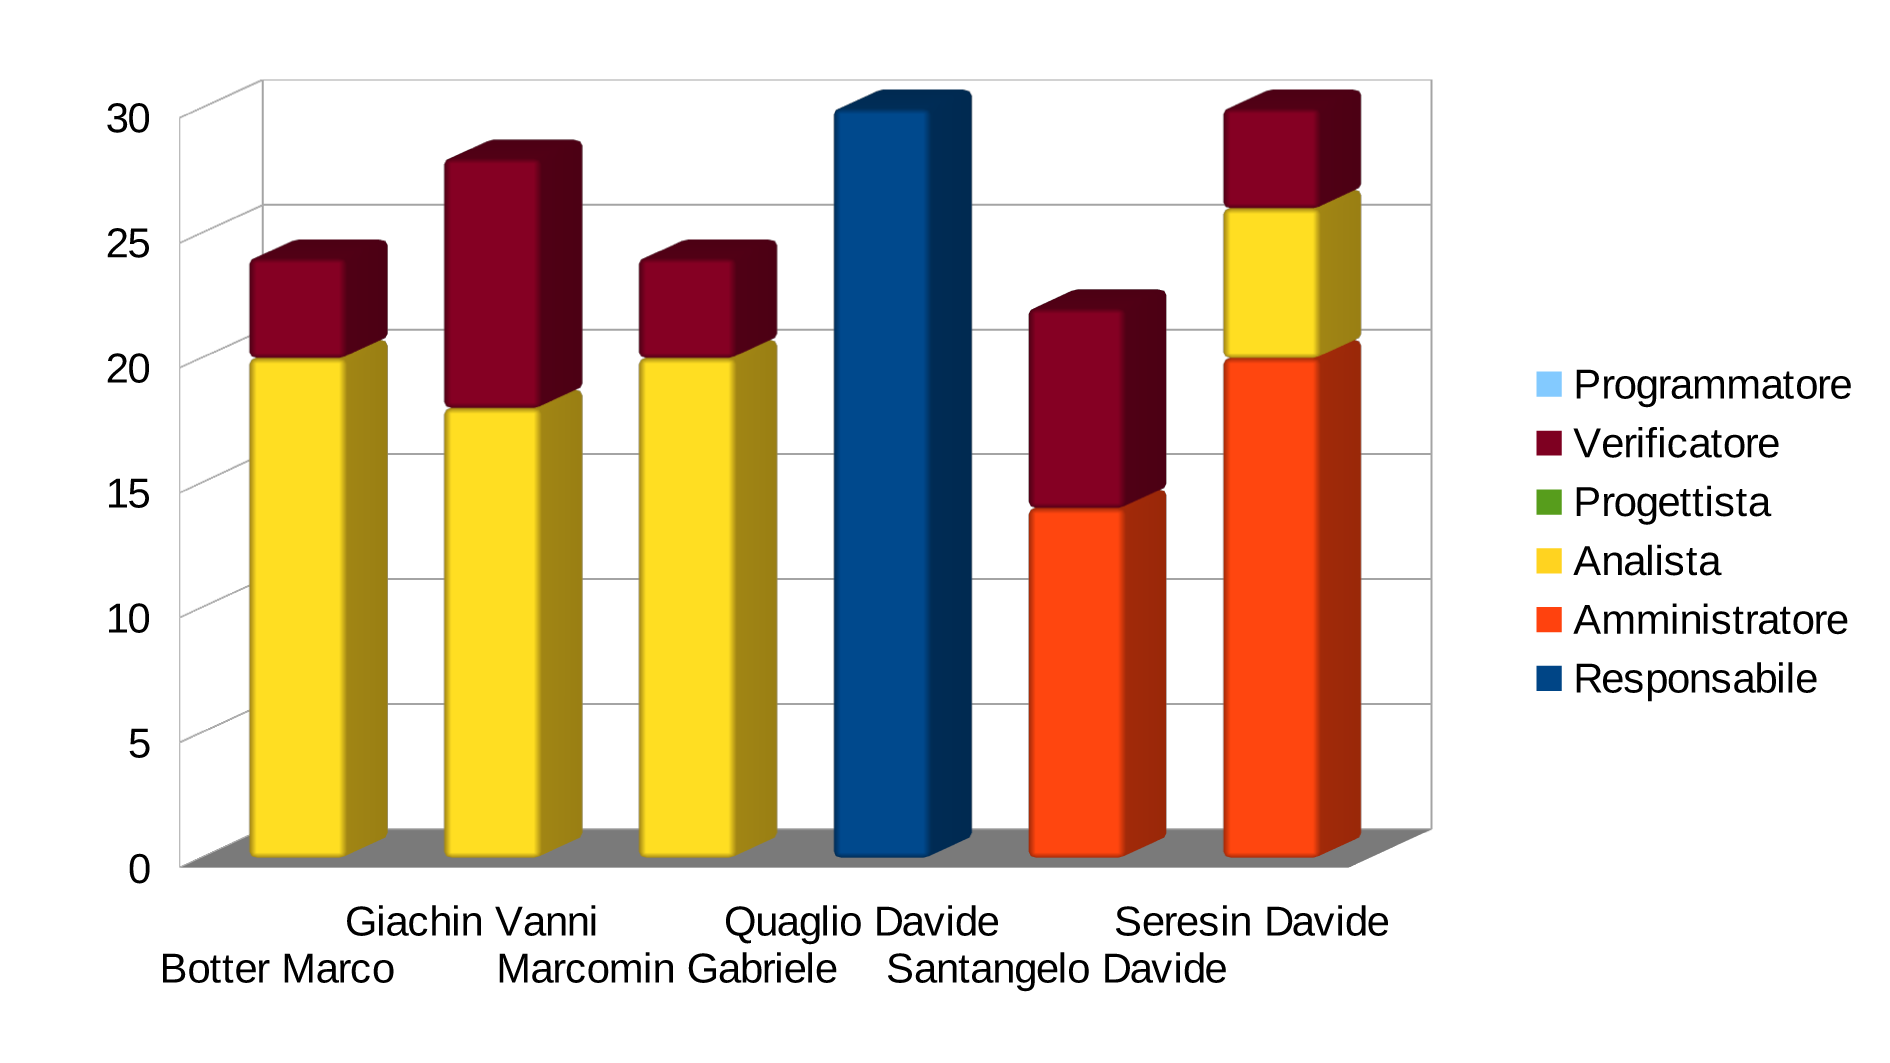
\includegraphics[scale=0.7]{../modello/img/1.png}}
        \end{picture}
\begin{center}
Grafico 1: Ore per componente periodo di Analisi.
\end{center}
\subsubsection{Prospetto economico}
\begin{center}
\begin{tabular}{| l | c | c |}
\hline
Ruolo & Ore & Costi \\
\hline
Responsabile & 30 & 900 \\
Amministratore & 34 & 680 \\
Analista & 64 & 1600 \\
Progettista & 0 & 0 \\
Verificatore & 30 & 450 \\
Programmatore & 0 & 0 \\
\hline
\textbf{Totale} & 158 & 3630 \\
\hline
\end{tabular}
\\
	Tabella 4: Tabella del prospetto economico.
\end{center}
\subsection{Progettazione Architetturale}
\subsubsection{Suddivisione dei ruoli}
\begin{center}
\begin{tabular}{| l | c | c | c | c | c | c | c |}
\hline
Membro & Re & Am & An & Pt & Ve & Pr & ore totali \\
\hline
Botter Marco & 10 & 0 & 3 & 12 & 4 & 0 & 29 \\

Giachin Vanni & 7 & 0 & 11 & 15 & 2 & 0 & 35 \\

Marcomin Gabriele & 10 & 4 & 4 & 11 & 4 & 0 & 33 \\

Quaglio Davide & 5 & 0 & 11 & 14 & 0 & 0 & 30 \\

Santangelo Davide & 0 & 2 & 13 & 0 & 10 & 0 & 25 \\

Seresin Davide & 6 & 0 & 6 & 15 & 2 & 0 & 29 \\
\hline
Ore totali & 38 & 6 & 48 & 67 & 22 & 0 & 181 \\
\hline
\end{tabular}
\\
Tabella 5: Ore per membro, periodo di Analisi
\end{center}
\setlength{\unitlength}{1mm}\begin{picture}(15,60)
                \put(10,0){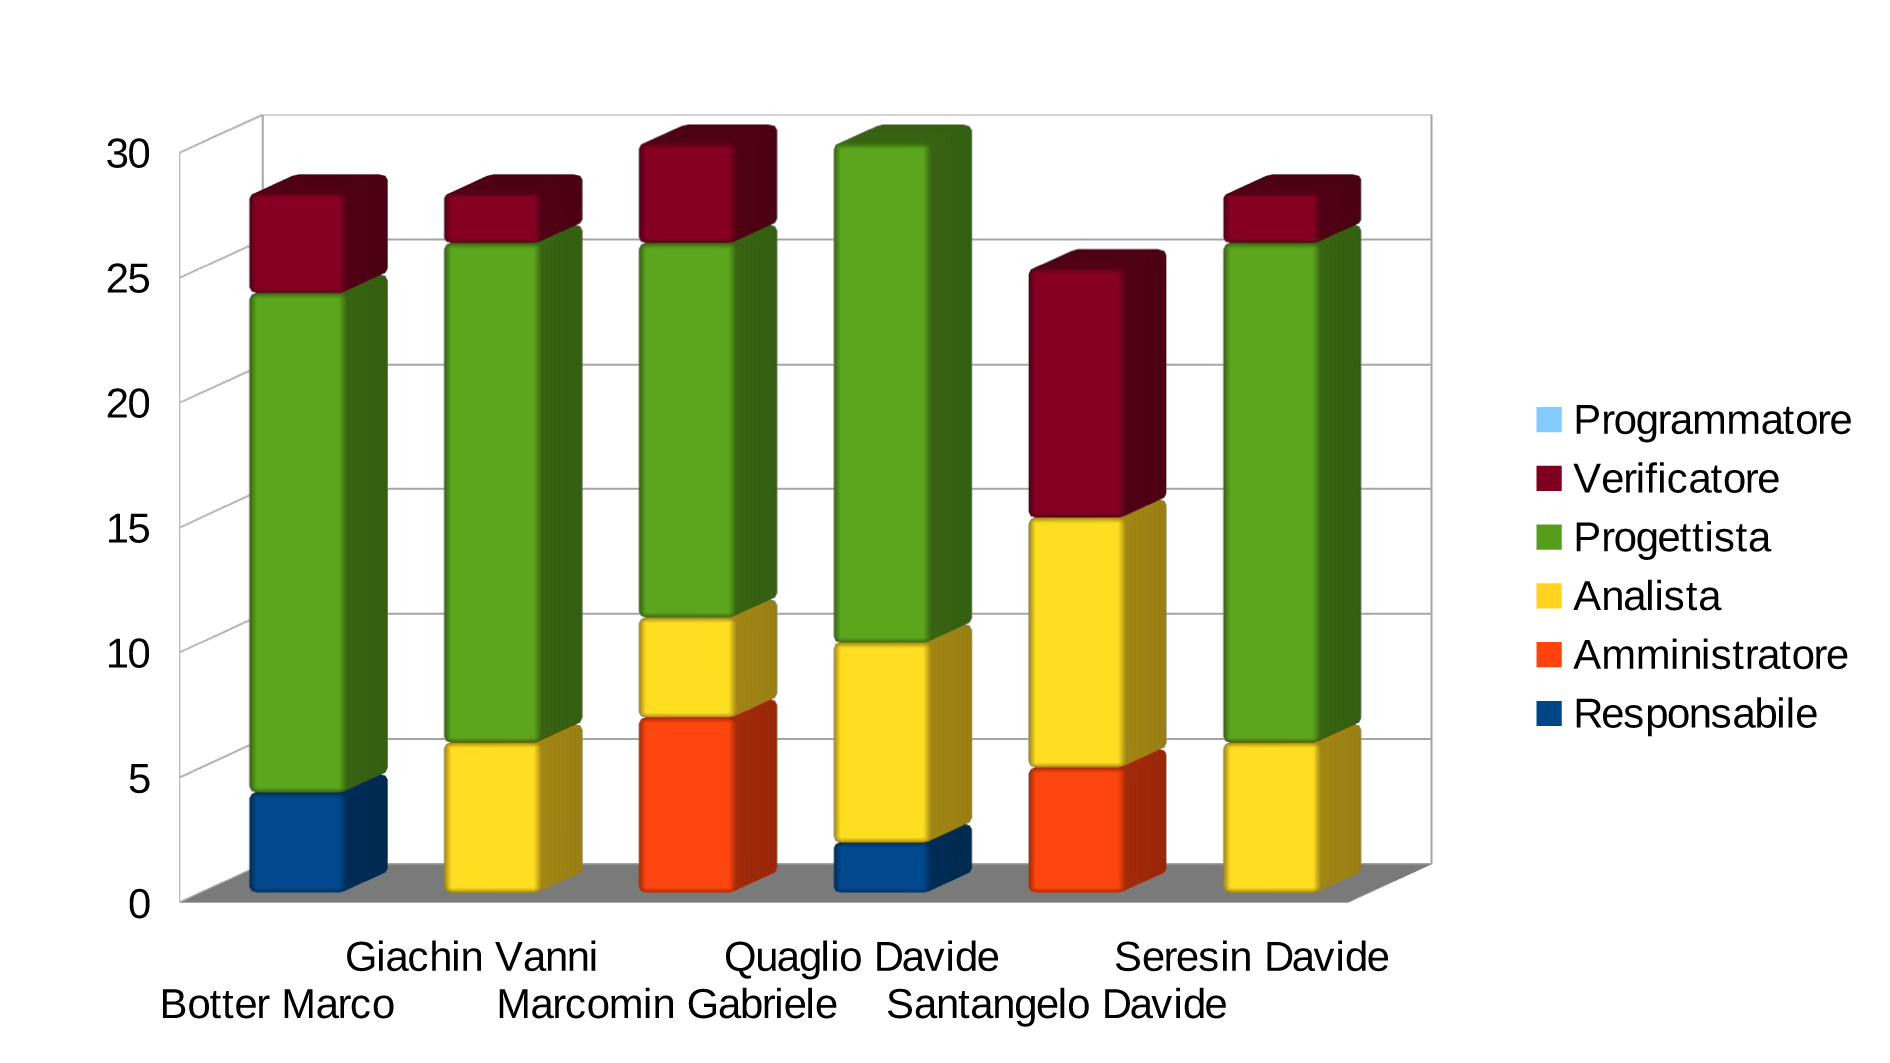
\includegraphics[scale=0.7]{../modello/img/2.png}}
        \end{picture}
\begin{center}
Grafico 2: Ore per componente periodo di Progettazione Architetturale.
\end{center}
\subsubsection{Prospetto economico}
\begin{center}
\begin{tabular}{| l | c | c |}
\hline
Ruolo & Ore & Costi \\
\hline
Responsabile & 38 & 1140 \\
Amministratore & 6 & 120 \\
Analista & 48 & 1200 \\
Progettista & 67 & 1474 \\
Verificatore & 22 & 330 \\
Programmatore & 0 & 0 \\
\hline
\textbf{Totale} & 181 & 4264 \\
\hline
\end{tabular}
\\
Tabella 6: Tabella del prospetto economico.
\end{center}
\subsection{Progettazione di Dettaglio e Codifica}
\subsubsection{Suddivisione dei ruoli}
\begin{center}
\begin{tabular}{| l | c | c | c | c | c | c | c |}
\hline
Membro & Re & Am & An & Pt & Ve & Pr & ore totali \\
\hline
Botter Marco & 10 & 0 & 0 & 13 & 14 & 8 & 45 \\

Giachin Vanni & 11 & 0 & 0 & 12 & 12 & 11 & 46 \\

Marcomin Gabriele & 14 & 0 & 0 & 0 & 15 & 15 & 44 \\

Quaglio Davide & 0 & 8 & 2 & 15 & 17 & 15 & 57 \\

Santangelo Davide & 0 & 0 & 3 & 22 & 15 & 15 & 55 \\

Seresin Davide & 0 & 0 & 0 & 19 & 20 & 0 & 39 \\
\hline
Ore totali & 35 & 8 & 5 & 81 & 93 & 64 & 286 \\
\hline
\end{tabular}
\\
Tabella 7: Ore per membro, periodo di Progettazione di dettaglio e codifica
\end{center}
\setlength{\unitlength}{1mm}\begin{picture}(15,60)
                \put(10,0){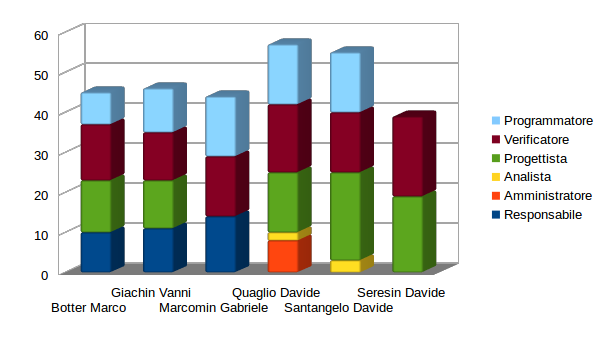
\includegraphics[scale=0.7]{../modello/img/3.png}}
        \end{picture}
\begin{center}
Grafico 3: Ore per componente periodo di Progettazione di Dettaglio e Codifica.
\end{center}
\subsubsection{Prospetto economico}
\begin{center}
\begin{tabular}{| l | c | c |}
\hline
Ruolo & Ore & Costi \\
\hline
Responsabile & 35 & 1050 \\
Amministratore & 8 & 160 \\
Analista & 5 & 125 \\
Progettista & 81 & 1782 \\
Verificatore & 93 & 1395 \\
Programmatore & 64 & 960 \\
\hline
\textbf{Totale} & 286 & 5472 \\
\hline
\end{tabular}
\\
Tabella 8: Tabella del prospetto economico.
\end{center}
\subsection{Verifica e Validazione}
\subsubsection{Suddivisione dei ruoli}
\begin{center}
\begin{tabular}{| l | c | c | c | c | c | c | c |}
\hline
Membro & Re & Am & An & Pt & Ve & Pr & ore totali \\
\hline
Botter Marco & 0 & 10 & 0 & 0 & 17 & 5 & 32 \\

Giachin Vanni & 0 & 10 & 0 & 0 & 15 & 0 & 25 \\

Marcomin Gabriele & 0 & 0 & 0 & 17 & 12 & 0 & 29 \\

Quaglio Davide & 6 & 0 & 0 & 0 & 13 & 0 & 19 \\

Santangelo Davide & 12 & 0 & 0 & 4 & 10 & 0 & 26 \\

Seresin Davide & 15 & 0 & 0 & 3 & 10 & 10 & 38 \\
\hline
Ore totali & 33 & 20 & 0 & 24 & 77 & 15 & 169\\
\hline
\end{tabular}
\\
Tabella 9: Ore per membro, periodo di Verifica e Validazione.
\end{center}
\setlength{\unitlength}{1mm}\begin{picture}(15,60)
                \put(10,0){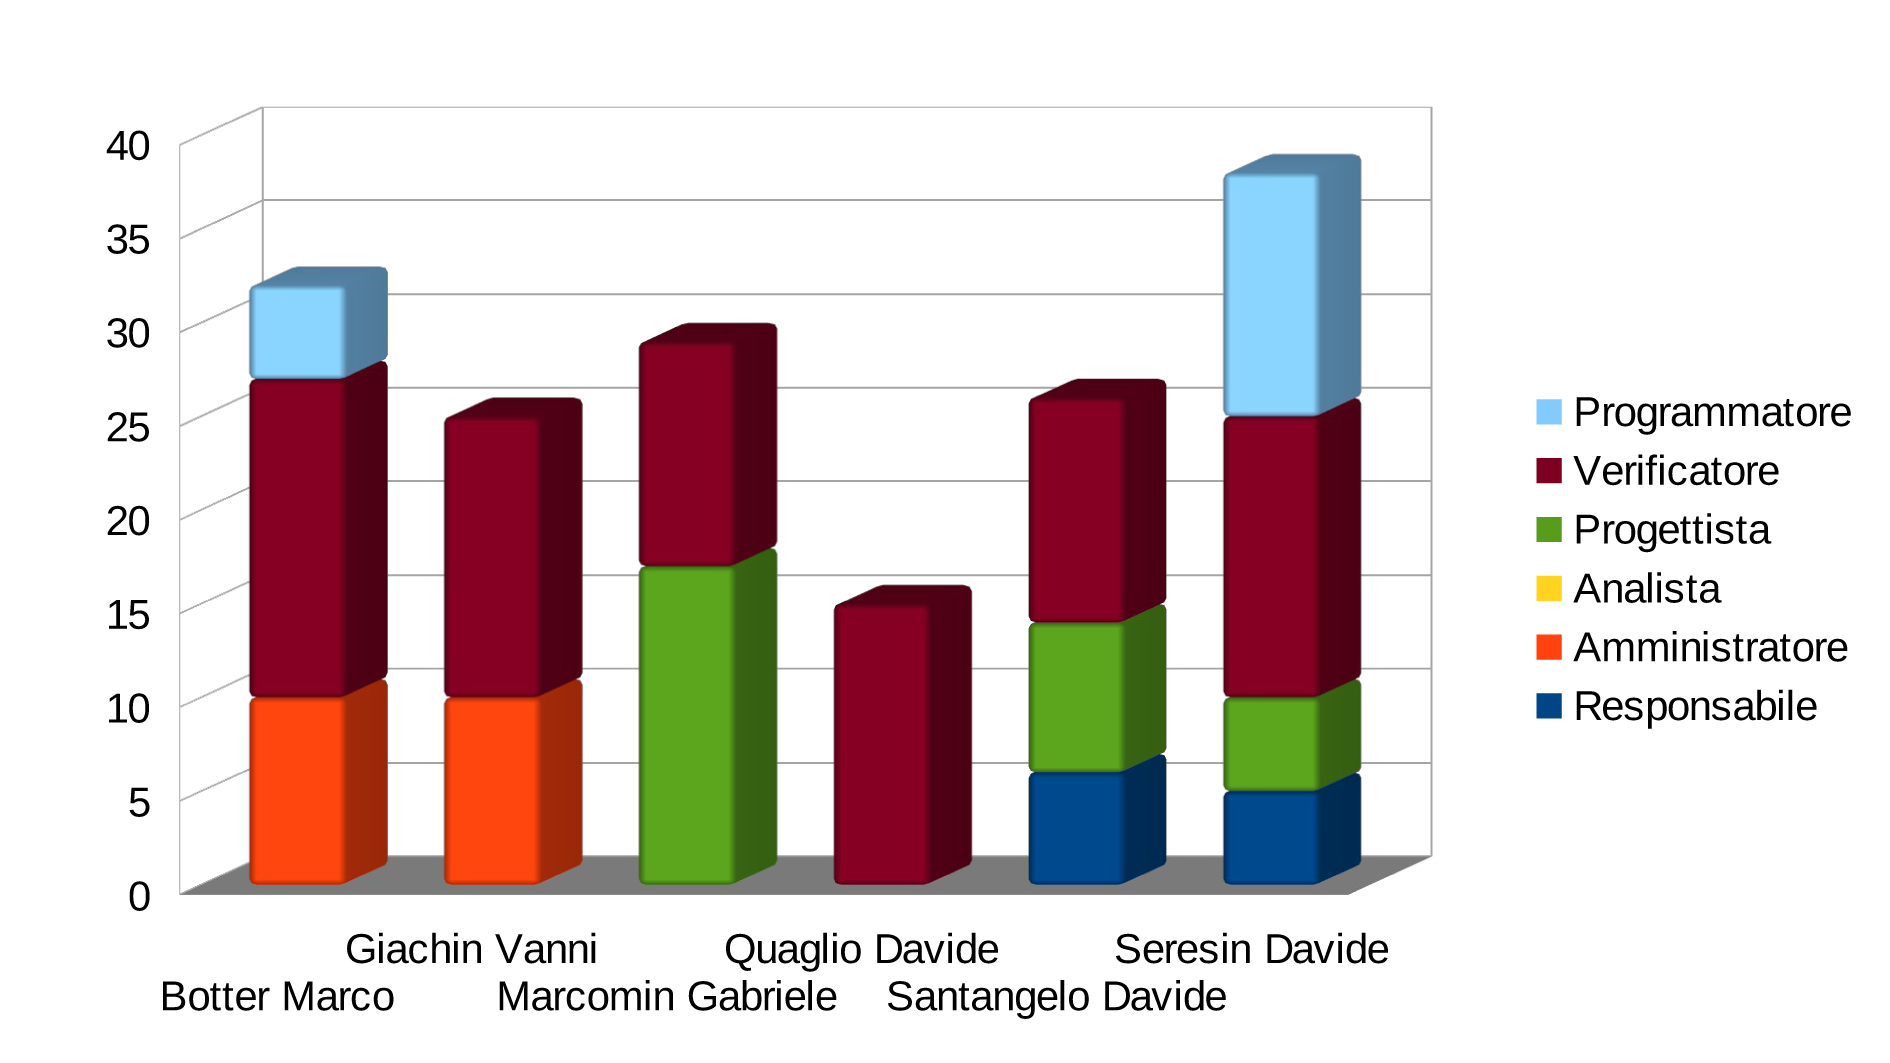
\includegraphics[scale=0.7]{../modello/img/4.png}}
        \end{picture}
\begin{center}
Grafico 4: Grafico ore per componente periodo di Analisi e Verifica.
\end{center}
\subsubsection{Prospetto economico}
\begin{center}
\begin{tabular}{| l | c | c |}
\hline
Ruolo & Ore & Costi \\
\hline
Responsabile & 33 & 990 \\
Amministratore & 20 & 400 \\
Analista & 0 & 0\\
Progettista & 24 & 528 \\
Verificatore & 77 & 1155 \\
Programmatore & 15 & 225 \\
\hline
\textbf{Totale} & 169 & 3298 \\
\hline
\end{tabular}
\\
Tabella 10: Tabella del prospetto economico.
\end{center}
\subsection{Totale}
\subsubsection{Suddivisone dei ruoli con periodo di Analisi}
Qui di seguito vengono riportate le ore dedicate da ogni compontente del gruppo \gruppo al progetto il \progetto:
\begin{center}
\begin{tabular}{| l | c | c | c | c | c | c | c |}
\hline
Membro & Re & Am & An & Pt & Ve & Pr & ore totali \\
\hline
Botter Marco & 20 & 10 & 23 & 25 & 39 & 13 & 130 \\

Giachin Vanni & 18 & 10 & 29 & 27 & 39 & 11 & 134 \\

Marcomin Gabriele & 24 & 4 & 24 & 28 & 35 & 15 & 130 \\

Quaglio Davide & 41 & 8 & 13 & 29 & 30 & 15 & 136 \\

Santangelo Davide & 12 & 16 & 16 & 26 & 43 & 15 & 128 \\

Seresin Davide & 21 & 20 & 12 & 37 & 36 & 10 & 136 \\
\hline
Ore totali & 136 & 68 & 117 & 172 & 222 & 89 & 794 \\
\hline
\end{tabular}
\\
Tabella 11: Ore per membro, periodo di Analisi
\end{center}
\setlength{\unitlength}{1mm}\begin{picture}(15,64)
                \put(10,0){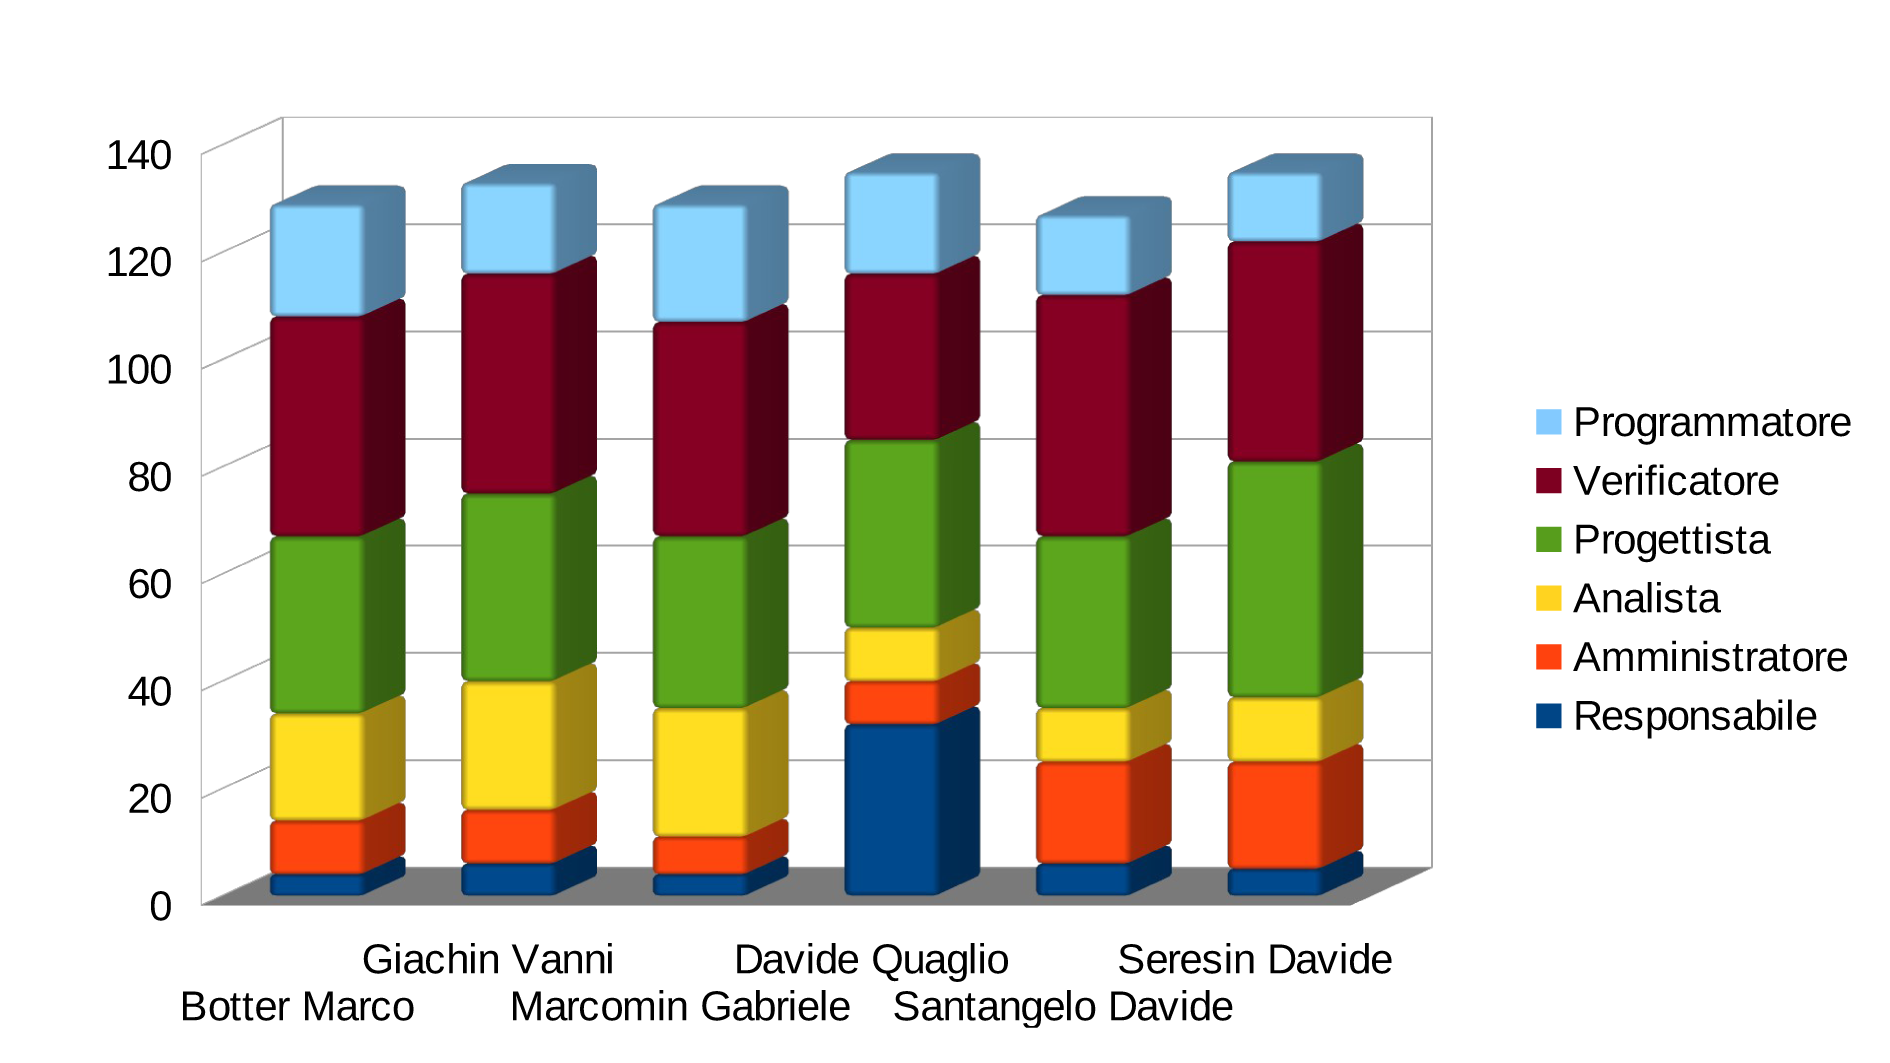
\includegraphics[scale=0.7]{../modello/img/5.png}}
        \end{picture}
\begin{center}
Grafico 5: Grafico ore per componente sul totale.
\end{center}
\subsubsection{Prospetto economico con periodo di Analisi}
\begin{center}
\begin{tabular}{| l | c | c |}
\hline
Ruolo & Ore & Costi \\
\hline
Responsabile & 136 & 4080 \\
Amministratore & 68 & 1360 \\
Analista & 117 & 2925\\
Progettista & 172 & 3784 \\
Verificatore & 222 & 3330 \\
Programmatore & 79 & 1185 \\
\hline
\textbf{Totale} & 794 & 16664 \\
\hline
\end{tabular}
\\
Tabella 11: Tabella del prospetto economico.
\end{center}
\setlength{\unitlength}{1mm}\begin{picture}(15,64)
                \put(10,0){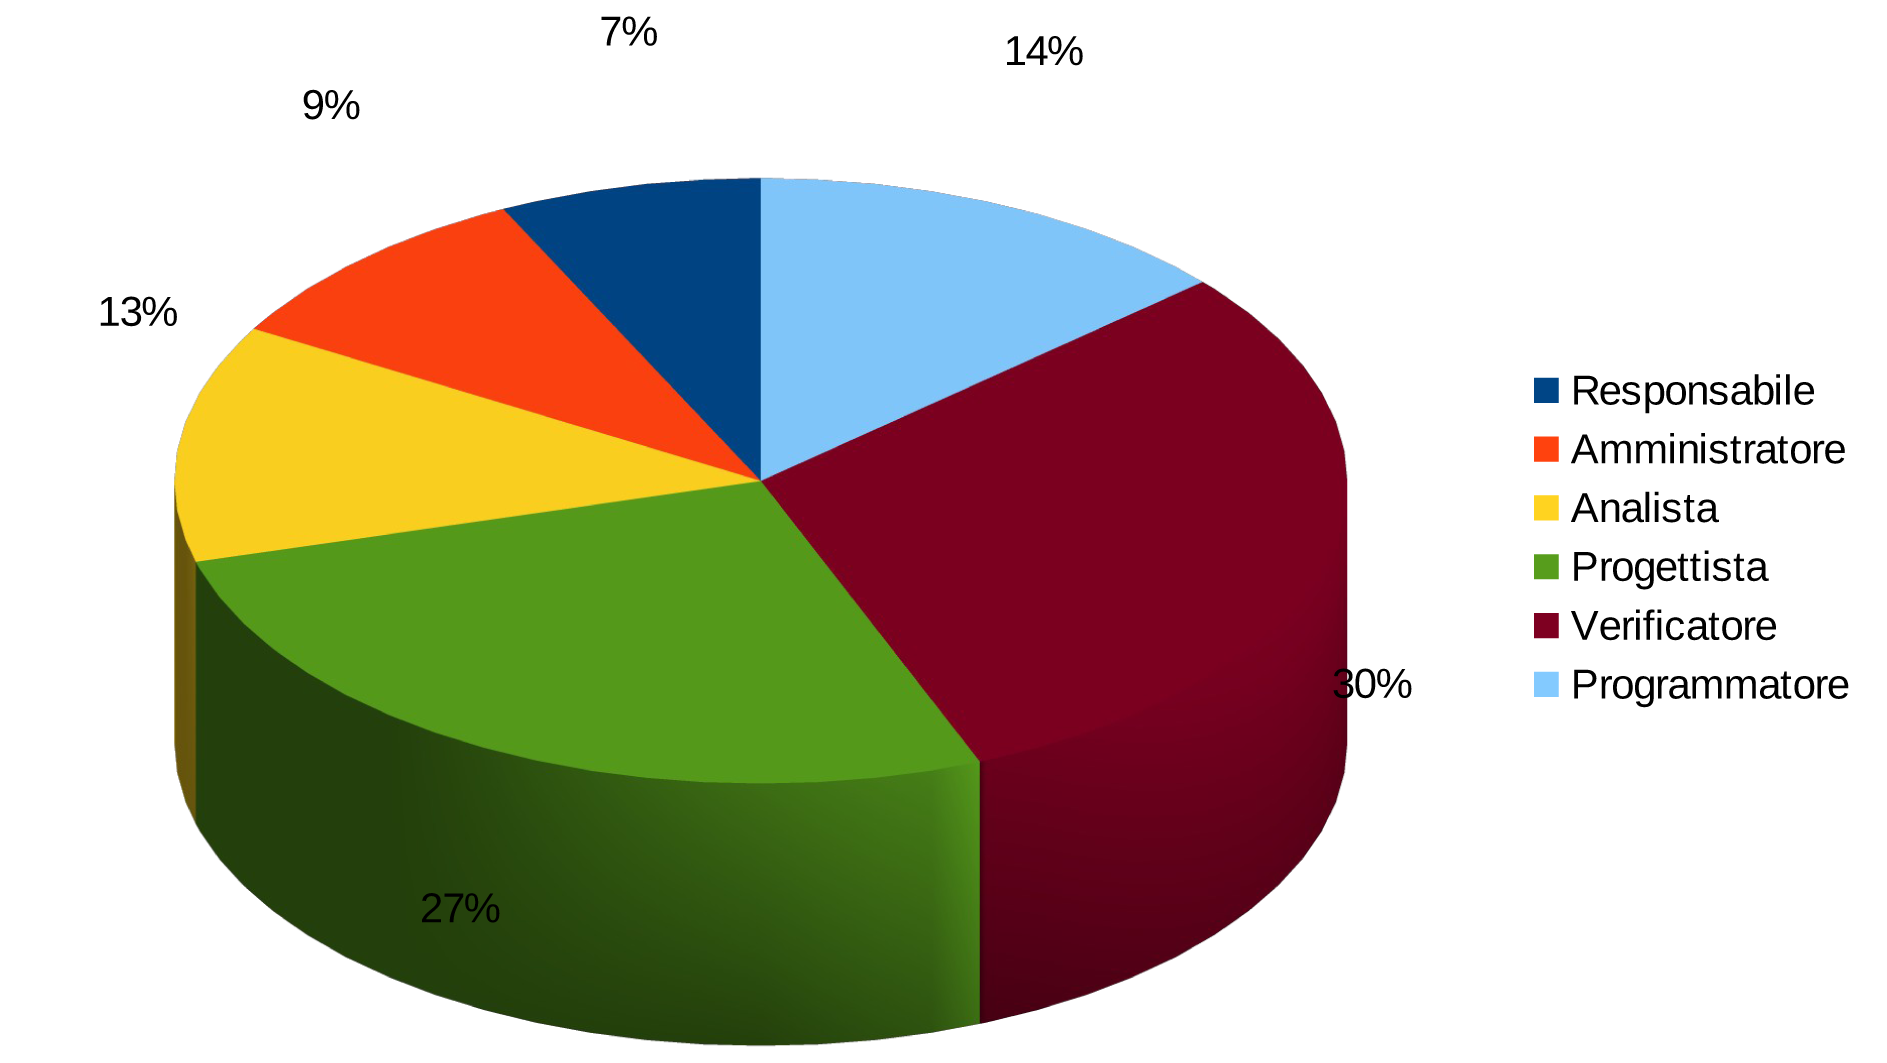
\includegraphics[scale=0.7]{../modello/img/torta5.png}}
    \end{picture}
\begin{center}
Grafico 6: Grafico sulla suddivisione dei compiti.
\end{center}
Si noti come le ore dedicate all'attività di verifica siano del 30\%.\\
\subsection{Ore rendicontate}
\subsubsection{Prospetto economico}
Per la realizzazione del progetto il team \gruppo{} ha stimato un costo totale che viene calcolato seguendo quanto riportato nella seguente tabella:
\begin{center}
\begin{tabular}{| l | c | c |}
\hline
Ruolo & Ore & Costi \\
\hline
Responsabile & 106 & 3180 \\
Amministratore & 34 & 680 \\
Analista & 53 & 1325\\
Progettista & 172 & 3784 \\
Verificatore & 192 & 2880 \\
Programmatore & 79 & 1185 \\
\hline
\textbf{Totale} & 636 & 13034 \\
\hline
\end{tabular}
\\
Tabella 12: Tabella del prospetto economico senza analisi.
\end{center}
Secondo i risultati ottenuti dalla tabella il costo totale per lo sviluppo del progetto è \textbf{13034}\euro .